\subsection{Correção da Abertura do Gol Devido a Movimentação da Bola}

Somente o ajuste de movimentação da bola foi anulado.  Os resultados no
planejamento são apresentados na Figura~\ref{fig:kickpos_0}.  Conforme pode ser
observado, a sombra dos robôs é maior, reduzindo assim abertura do gol.  Logo,
poucos robôs são necessários para bloquear o gol.  Isso gerou mais ações
direcionadas para posições de ataque.

\begin{figure}[H]
  \centering
  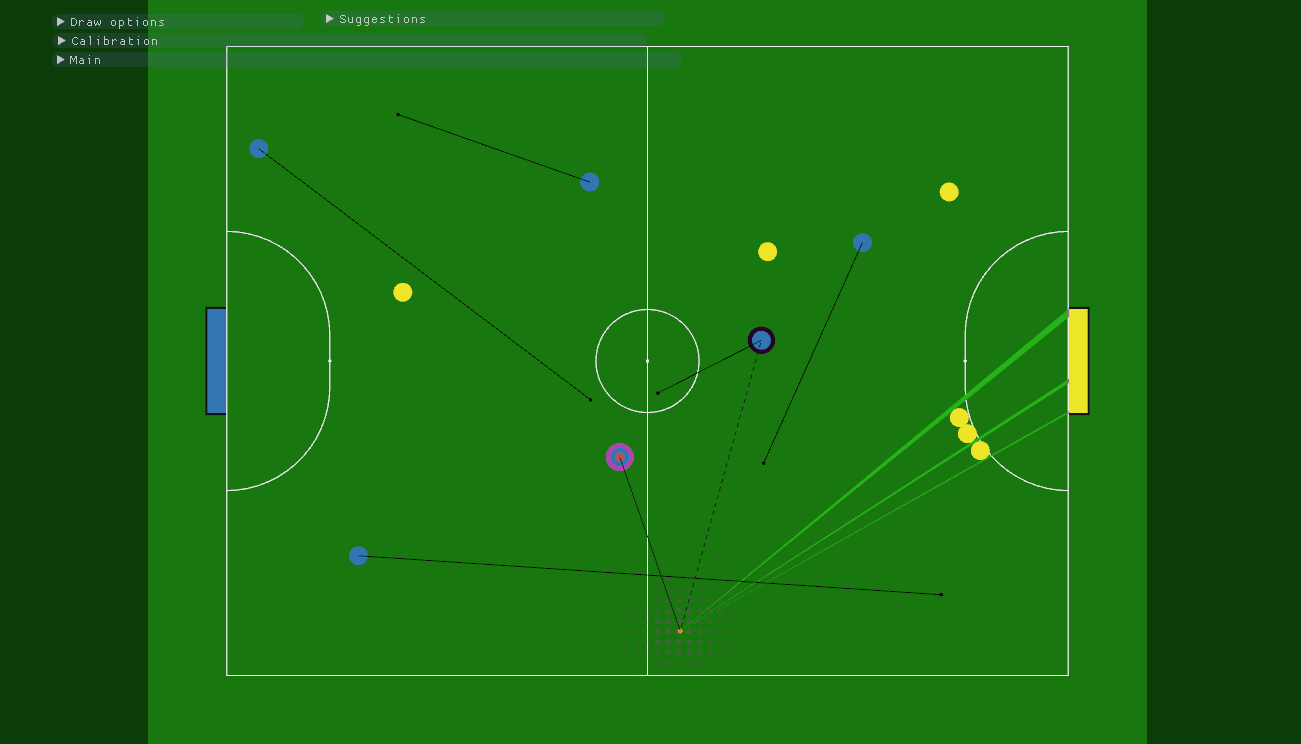
\includegraphics[width= 0.8\linewidth]{result/kickpos_0_atq}
  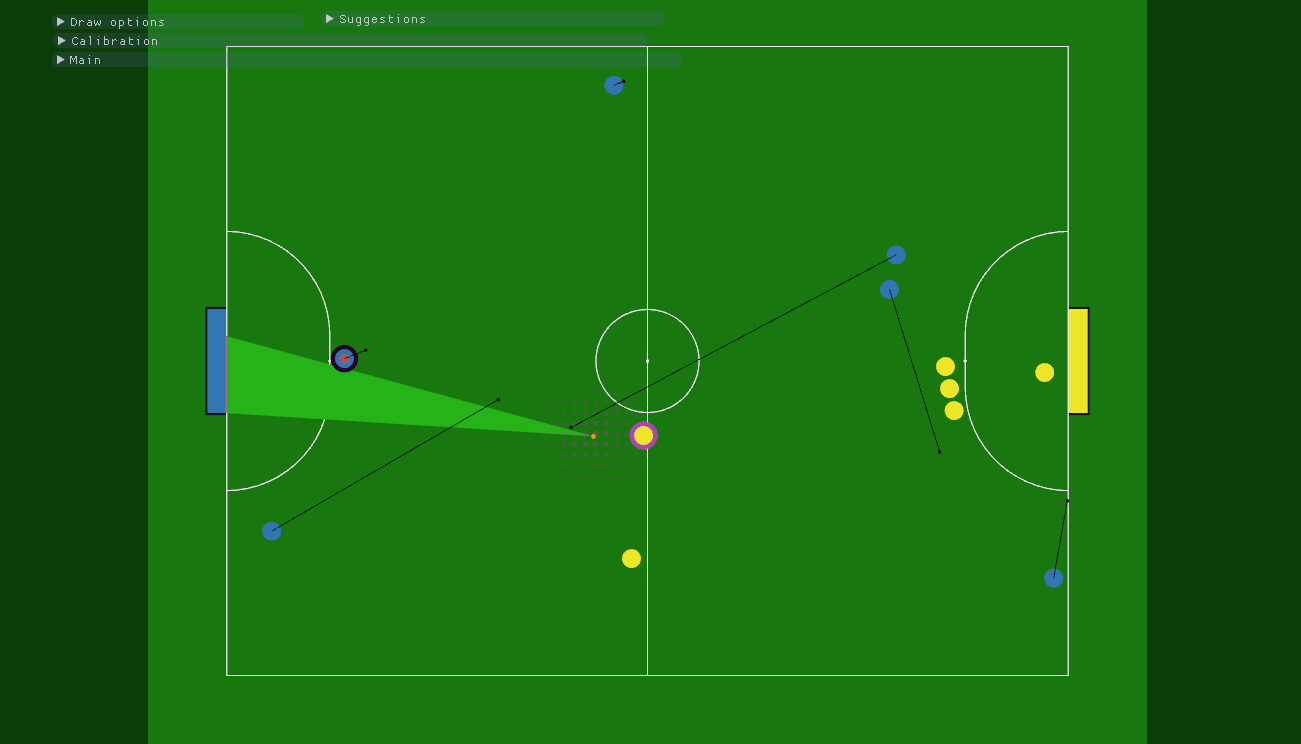
\includegraphics[width= 0.8\linewidth]{result/kickpos_0_def}
  \caption{Planejamento com os parâmetros inicias e sem ajuste de movimentação
  da bola em ambiente de ataque (acima) e defesa (abaixo)}\label{fig:kickpos_0}
\end{figure}

Depois esse ajuste foi alterado para $0.24$.  Os resultados em ambiente de
ataque e defesa são apresentados na Figura~\ref{fig:kickpos_024}.  A sombra de
cada robô é menor, resultando em mais robôs próximos ao gol para reduzir a
abertura do gol vista pelos robôs adversários.

\begin{figure}[H]
  \centering
  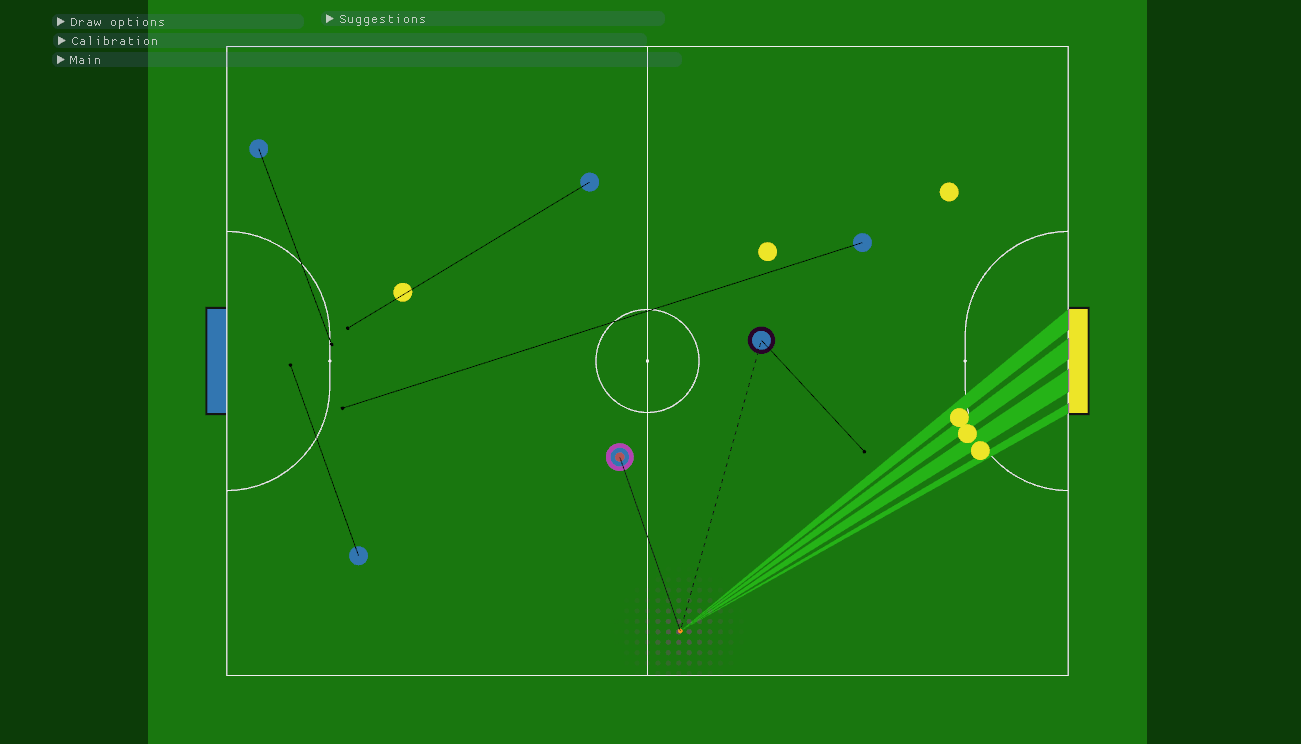
\includegraphics[width= 0.8\linewidth]{result/kickpos_024_atq}
  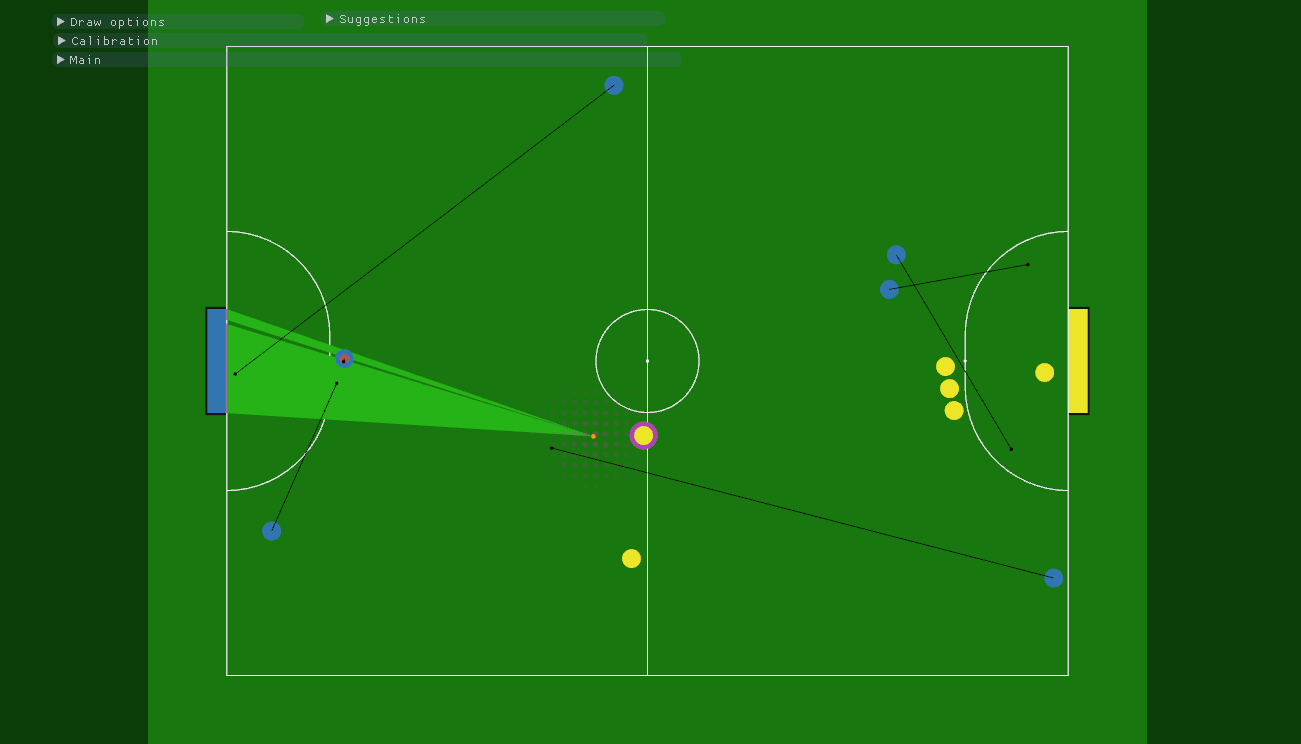
\includegraphics[width= 0.8\linewidth]{result/kickpos_024_def}
  \caption{Planejamento com os parâmetros inicias e o ajuste de movimentação da
  bola ajustado para $0.24$ em ambiente de ataque (acima) e defesa (abaixo)}\label{fig:kickpos_024}
\end{figure}

% vim: tw=80 et ts=2 sw=2 sts=2 ft=tex spelllang=pt_br,en
